\begin{figure}[t]
\centering
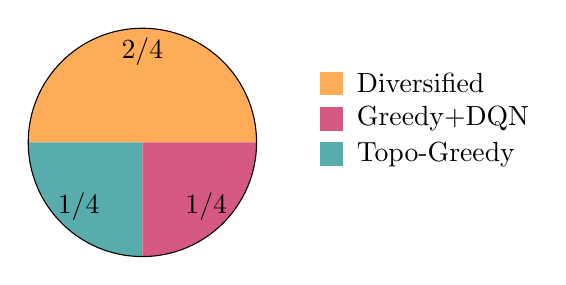
\begin{tikzpicture}[x=1cm,y=1cm]
\fill[orange!65] (0,0) -- (0.00:1.45) arc (0.00:180.00:1.45) -- cycle;
\node at (0.00,1.15) {2/4};
\fill[teal!65] (0,0) -- (180.00:1.45) arc (180.00:270.00:1.45) -- cycle;
\node at (-0.81,-0.81) {1/4};
\fill[purple!65] (0,0) -- (270.00:1.45) arc (270.00:360.00:1.45) -- cycle;
\node at (0.81,-0.81) {1/4};
\draw (0,0) circle (1.45);
\fill[orange!65] (2.25,0.60) rectangle (2.55,0.90); \node[right] at (2.60,0.75) {Diversified};
\fill[purple!65] (2.25,0.15) rectangle (2.55,0.45); \node[right] at (2.60,0.30) {Greedy+DQN};
\fill[teal!65] (2.25,-0.30) rectangle (2.55,-0.00); \node[right] at (2.60,-0.15) {Topo-Greedy};
\end{tikzpicture}
\caption{Adaptive TACC policy-selection frequency across the four perturbation regimes. The cost-aware selector uses topology-aware greedy when DQN's marginal gain is too small to justify added computation, diversified placement in moderate perturbation, and DQN refinement when high-churn instability makes refinement worthwhile.}
\label{fig:generated_selector_pie}
\end{figure}
